%-------------------------------------------------------------------------------
\chapter[Mixed sediment]{Mixed sediment transport}
%-------------------------------------------------------------------------------

%-------------------------------------------------------------------------------
\section{Preliminaries}
%-------------------------------------------------------------------------------
Natural  sediments  in  estuaries  and  coastal  areas  are  usually characterised  by  a  mixture  of water, sand, mud and organic matters. This heterogeneity can be modeled by a mixing of cohesive and  non-cohesive sediments. A sand-mud mixture can be therefore represented by two classes of bed material: the mud fraction, which represents the slower settling species and the sand fraction, which represents the faster settling species~\cite{Lan12}.

\textbf{So far it is assumed only suspended load,
which implies that the model solves mixtures of fine sand grains and
mud}.

Two sediment classes are considered to solve sediment mixtures. The first class (noted $1$) is \textbf{non-cohesive sediment} and is represented by its grain diameter $D_1$. The
settling velocity $w_{s1}$ is a function of the relative sediment density
($s=1.65$) and grain diameter $D_1$. 

The second class (noted $2$) is \textbf{cohesive sediment}, with grain diameter $D_2$ less than $60$
$\mu$m. The settling velocity $w_{s2}$ is a function of flocs properties which
differs from the individual cohesive particles, and needs to be specified. 

The sediment mixture is divided into two size classes $k=1,2$. As only the suspended sediment transport is considered, the depth-averaged transport equation of the $k$th size class of sediment is:

\begin{equation}\label{eq:ADE}
\frac{\partial hC_k}{\partial t} + \frac{\partial hUC_k}{\partial
x} + \frac{\partial hVC_k}{\partial y} =\frac{\partial }{%
\partial x} \left(h\epsilon_s\frac{\partial C_k}{\partial x} \right) +%
\frac{\partial }{\partial y} \left( h\epsilon_s\frac{\partial C_k}{%
\partial y} \right)+E^k - D^k, 
\end{equation}%
where $C_k$ is the depth-averaged concentration of the $k$th size class of sediment, $\epsilon_s$ is the eddy viscosity, $E^k$ is the erosion rate and $D^k$ is the deposition rate. In the following, index $i$ stands for number of nodes, index $j$ stands for number of layers and index $k$ stands for number of classes ($k=1,2$ for sand and mud respectively).\\

\subsection{Limitations of the current version} 
\begin{itemize}
\item Only one sediment size is allowed for the sand, with constant density for all layers: the volume percentage can vary for different layers.
\item Only one sediment size is allowed for the mud: the mass concentration and volume percentage can vary for different layers.
\item The consolidation of the sand/mud mixture has not been yet implemented.
\end{itemize}

\subsection{Mixed sand-mud sediment model} 

The bed layer thickness and the mass of sand and mud (respectively $E_{s_j}^1$, $E_{s_j}^2$ and $M_{s_j}^1$, $M_{s_j}^2$) are first initialized for each layer. The mass of sand per layer, expressed in [kg/m$^2$], is computed as $M_{s_j}^1=E_{s_j}^1\rho_s$, with $\rho_s$ the sediment density. The mass of mud, expressed in mass per unit surface area [kg/m$^2$], is computed as $M_{s_j}^2=E_{s_j}^2 C_j$, with $C_j$ the mass concentration per layer [kg/m$^3$]. 

\subsubsection{Mean bed shear strength}
The mean bed shear strength per layer $\bar \tau_{ce_j}$ of the sand-mud mixture is computed for each layer as a function of the mass percentage of mud $f_{2_j}=M_{s_j}^2/(M_{s_j}^1+M_{s_j}^2)$:
\begin{itemize}
\item If $f_{2_j} \leq 30\%$ (sand dominant), then $\bar \tau_{ce_j} = \tau_{ce}^1$, with $\tau_{ce}^1$ the shear stress for sand, computed from the subroutine \texttt{init\_sediment.f}.
\item If $f_{2_j} \geq 50\%$ (mud dominant), then $\bar \tau_{ce_j} = \tau_{ce_j}^2$, with $\tau_{ce_j}^2$ the shear stress for mud, is provided by the keyword \texttt{CRITICAL EROSION SHEAR STRESS OF THE MUD} (real list, set to \texttt{0.01;0.02;0.03;...} by default), expressed in [N/m$^2$].
\item If $30\% < f_{2_j} < 50\%$, a linear interpolation is assumed:
\begin{equation}
\bar \tau_{ce_j} = \tau_{ce}^1 + \frac{(f_{2_j}-0.30)(\tau_{ce_j}^2-\tau_{ce}^1)}{(0.50-0.30)}.
\end{equation}
\end{itemize}

\begin{figure}[H]
\begin{center}
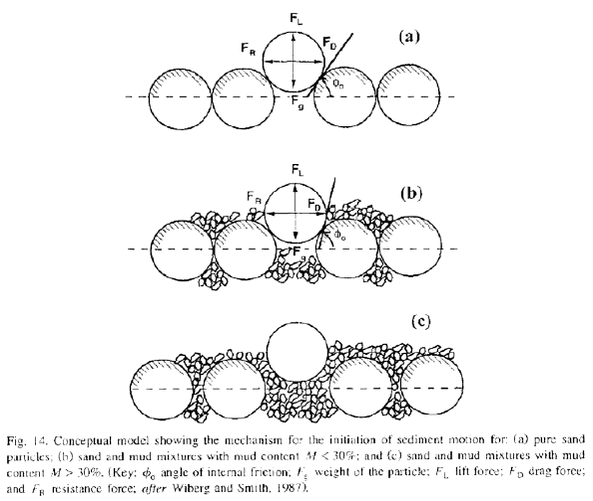
\includegraphics[trim=0cm 2.5cm 0cm 0cm, clip=true, scale=0.5,angle=0]{graphics/Mixed-fig001.png}
\caption{Conceptual model showing the mechanism for the initiation of sediment motion for: (a) sand only; (b) sand and mud mixture with mud content $f_2 < 30\%$; (c) sand and mud mixture with mud content $f_2 > 50\%$. In the picture, $\phi_0$ is the angle of internal friction; $F_g$ is the weight of the particle; $F_L$ is the lift force; $F_D$ is the drag force and $F_R$ is the resistance force~\cite{deLinaresthesis}.}\label{fig:mixed_regime}
\end{center}
\end{figure}

\subsubsection{Mean erosion flux per layer}
The erosion flux depends on the sediment composition of the bed layer. The mean erosion rate per layer $\bar E_j$ is determined as follows:
\begin{itemize}
\item If $f_{2_j} \leq 30\%$ (sand dominant), then the equilibrium concentration is assumed:
\begin{equation*}
\bar E_j = E_j^1 = \left\{\begin{array}{ll}
w_{s1} C_{eq} f_{1_1} \quad & \text{if}\,\,\tau_b>\bar \tau_{ce_j}\\  
0\quad & \text{otherwise},
\end{array}
\right. 
\end{equation*}
with $f_{1_1}$ the volume percent of sand contained in the first layer, 
$\tau_b$ the bottom shear stress and the equilibrium concentration $C_{eq}$, computed as presented in \S\ref{sec:concform}. 
\item If $f_{2_j} \geq 50\%$ (mud dominant), then the Krone-Partheniades erosion law is assumed:
\begin{equation*}
\bar E_j = E_j^2 = \left\{\begin{array}{ll}
M\left[\left(\frac{\tau_b}{\bar \tau_{ce_j}}\right)-1\right]\quad & \text{if}\,\,\tau_b>\bar \tau_{ce_j}\\  
0\quad & \text{otherwise},
\end{array}
\right. 
\end{equation*}
with $M$ the Krone-Partheniades erosion law constant [kg/m$^2$/s], provided by the keyword \texttt{PARTHENIADES CONSTANT} (real variable, set to \texttt{1.E-03} by default).

\item If $30\% < f_{2_j} < 50\%$, then a linear interpolation is assumed:
\begin{equation*}
\bar E_j = E_j^1 + \frac{(f_{2_j}-0.30)(E_j^2-E_j^1)}{(0.50-0.30)}.
\end{equation*}

\end{itemize}

\subsubsection{Sand and mud deposition fluxes}
Deposition fluxes for sand $D^1$ and mud $D^2$ used in the advection-diffusion equation (\ref{eq:ADE}) are computed as:
\begin{itemize}
\item For sand:
\begin{equation}
D^1 = w_{s1} T_2, 
\end{equation}
with $T_2$ the ratio between the near bed concentration and the mean concentration, computed by the subroutine \texttt{suspension\_rouse}. 

\item For mud:
\begin{equation}
D^2 = w_{s2} \left[1-\left(\frac{T_1}{u_{*mud}^{cr}}\right)^2 \right],
\end{equation}
with $u_{*mud}^{cr}$ the critical shear velocity for mud deposition [m/s] provided by the keyword \texttt{CRITICAL SHEAR VELOCITY FOR MUD DEPOSITION} (real variable, set to \texttt{1000.} by default) and $T_1=\sqrt{\tau_b/\rho}$.

\end{itemize}

\section{Steering file setup for a mixed sediment distribution (sand-mud)}\label{sec:}
Mixed sediment processes (sand and mud) are set in the \sisyphe{} steering file with the keyword
{\ttfamily MIXED SEDIMENT = YES} (logical variable, set to {\ttfamily = NON} by default). To secure the procedure, it is recommendable to set the following keywords as follows:
\begin{itemize}
\item {\ttfamily BED LOAD = NON}
\item {\ttfamily SUSPENSION = YES}
\item {\ttfamily COHESIVE SEDIMENTS = NON}  
\end{itemize}

The mixed sediment distribution (sand-mud) must be set with the keyword {\ttfamily NUMBER OF SIZE-CLASSES OF BED MATERIAL = 2} (integer type variable, set to {\ttfamily = 1}). Typically, the following variables can be specified in the steering file:

\begin{itemize}
\item Mean diameter {\ttfamily SEDIMENT DIAMETERS} (real type list, set to {\ttfamily = 0.01} m by default) must be set as follows:\\
{\ttfamily SEDIMENT DIAMETERS = D1, D2}, where {\ttfamily D1} is the sediment diameter of the sand and {\ttfamily D2} is the sediment diameter of the mud.

\item The initial volume fraction in the mixture {\ttfamily INITIAL FRACTION FOR PARTICULAR SIZE CLASS} (real type list, set to {\ttfamily = 1.,0.,0.,...} by default) must be set as follows:\\
  
{\ttfamily INITIAL FRACTION FOR PARTICULAR SIZE CLASS = f1, f2}\\
where {\ttfamily f1} and {\ttfamily f2} are respectively the (initial) volume percent of sand and mud. The sum of the percentage of each class of material must always be equal to $1$.

\item Values of settling velocities for sand and mud can be specified with the keyword {\ttfamily SETTLING VELOCITIES = ws1, ws2}, where {\ttfamily ws1} and {\ttfamily ws2} are respectively the settling velocities for the sand and mud.

\item The critical Shields parameter for the sand can be provided by the user through the leyword \texttt{SHIELDS PARAMETERS} or computed by \sisyphe{} if not specified.

\item \texttt{CRITICAL EROSION SHEAR STRESS OF THE MUD} (real list with \texttt{NOMBLAY} elements, set to {\ttfamily = 0.01;0.02;0.03;...} by default), expressed in N/m$^2$.\\

\item \texttt{MUD CONCENTRATION PER LAYER} (real list, set to {\ttfamily = 50.;100.;...} by default), expressed in kg/m$^3$ or gr/l.

\item \texttt{CRITICAL SHEAR VELOCITY FOR MUD DEPOSITION} (real value, set to {\ttfamily = 1000.} by default), expressed in m/s.

\item \texttt{PARTHENIADES CONSTANT} (real value, set to {\ttfamily = 1.E-03} by default), expressed in kg/m$^2$/s.
\end{itemize}

Values of initial and boundary conditions are specified as described in \S\ref{sec:SuspendedSedimentTransport}.

\subsection{Bed structure: discretization by layers}
The mixed sediment bed can be represented by a fixed number of layers ($<20$) with the keyword \texttt{NUMBER OF LAYERS OF THE CONSOLIDATION MODEL}, (integer variable, set to {\ttfamily = 1} by default). This procedure is secured by including \texttt{MUD CONSOLIDATION = NON} (logical variable, set to {\ttfamily = NON} by default) in the steering file.\\

The initial layer distribution, concentration and fraction distribution for sand and mud can be specified in the subroutine \texttt{init\_compo\_coh.f}.\\

For each layer, the mud thickness \texttt{EPAI\_VASE(J), J= 1,NOMBLAY} (being \texttt{NOMBLAY} the number of layers $\geq 2$) can be provided.

The sand thickness \texttt{EPAI\_SABLE(J)} is computed as function of the initial sediment distribution of each class: if the initial distribution is constant (per layer and per node), the initial fraction of material can be specified with the keyword \texttt{INITIAL FRACTION FOR PARTICULAR SIZE CLASS} (variables $f_{1_1}$ \texttt{AVA0(1)} and $f_{2_1}$ \texttt{AVA0(2)} for sand and mud for the first layer, respectively).
More generally, the volume percent of each class for each layer can also be specified with the variables \texttt{AVAIL(I,J,1)} ($f_{1_j}$ for sand) and \texttt{AVAIL(I,J,2)} ($f_{2_j}$ for mud) for \texttt{I=1,NPOIN} and \texttt{J= 1,NOMBLAY}. The total thickness of each layer $E_{s_j} = E_{s_j}^1 + E_{s_j}^2$ can also be specified. 

The initial mass concentration by layer is provided in the variable \texttt{CONC(I,J)} for \texttt{I=1,NPOIN} and \texttt{J= 1,NOMBLAY}.


